%% !TEX root=main.tex
%% !TEX TS-program = XeLaTeX
% گزارش پروژه AI Mining
% پروژه استخراج داده با استفاده از هوش مصنوعی
%%%%%%%%%%%%%%%%%%%%%%%%%%%%%%%%%%%%%%%%
\documentclass[a4paper,oneside,12pt]{report}
%در صورت نیاز به فراخوانی بسته‌های اضافی، آن‌ها را در فایل commands.tex و قبل از
%بسته زی‌پرشین فراخوانی کنید.
\usepackage{threeparttable}
\include{SBUKThesis-commands}
%%%%%%%%%%%%%%%%%%%%%%%%%%%%5
%\PersianMathsDigits
% \usepackage[backend=biber,style=numeric,sorting=none]{biblatex}
% \addbibresource{bibliography.bib}

% تنظیمات زی‌پرشین
% \usepackage[extrafootnotefeatures]{xepersian}
% \settextfont[Scale=1.2]{XB Zar}
% \setdigitfont[Scale=1.2]{XB Zar}

\begin{document}
\pagenumbering{myabjad}
%در صورتی که می خواهید دو صفحه خالی در ابتدای گزارش باشد، دو خط زیر فعال شود
%\include{blankpage}
%\cleardoublepage
% !TeX root=main.tex
\setlength{\parindent}{0pt}
\begin{titlepage}
    \vspace*{\fill}
    \centering
    {\fontsize{18}{19}\selectfont\bfseries نوآوری‌های هوش مصنوعی در فرآوری مواد معدنی\par}
    \vspace{0.5cm}
    {\fontsize{14}{15}\selectfont به همراه رزومه و معرفی علیرضا ایرانمنش \par}
    
    \vspace{1cm}
    
    {\fontsize{16}{17}\selectfont\bfseries علیرضا ایرانمنش\par}
    \vspace{0.3cm}
    {\fontsize{14}{15}\selectfont دانشجوی کارشناسی ارشد هوش مصنوعی – دانشگاه شهید باهنر کرمان \par}
    
    \vspace*{\fill}
    {\fontsize{14}{15}\selectfont\bfseries شهریور ۱۴۰۴ \par}
    \vspace*{\fill}
\end{titlepage}%صفحه جلد
%%%%%%%%%%%%%%%%%%%%%%%%%%%
\tableofcontents%فهرست مطالب
\cleardoublepage
\setlength{\cftfignumwidth}{2.5em}
%\listoffigures%
{
	\let\oldnumberline\numberline%
	\renewcommand{\numberline}{\figurename~\oldnumberline}%
	\listoffigures%
}
\cleardoublepage
%%%%%%%%%%%%%%%%%%%%%%%%%%%%%%%%
\pagenumbering{arabic}
\titleformat{\chapter}[display]
{\vspace{5cm}\filcenter}
{\filcenter \LARGE\bfseries
\chaptertitlename\ \justwords{\thechapter}\!:}
{1ex}
{\filcenter\fontsize{24}{25}\selectfont\bfseries\thispagestyle{empty}}
[\vfill\clearpage]
\def\justwords#1{\ifcase#1 \or اول \or دوم \or سوم \or چهارم \or پنجم \or ششم \or هفتم etc.\fi}
%%%%%%%%%%
 \titleformat*{\section}{\bfseries\fontsize{13}{14}\selectfont}
\titleformat*{\subsection}{\bfseries\fontsize{12}{13}\selectfont}
\titleformat*{\subsubsection}{\bfseries\fontsize{11}{12}\selectfont}
%%%%%%%%%%%%%%%%%%%%%%%%%%%%%%%%
\setlength{\parindent}{20pt}
% !TeX root=main.tex
\chapter{معرفی شخصی}

اینجانب علیرضا ایرانمنش، فارغ‌التحصیل مقطع کارشناسی فناوری اطلاعات و دانشجوی کارشناسی‌ارشد رشته هوش مصنوعی در دانشگاه شهید باهنر کرمان هستم. 
به‌واسطه‌ی عملکرد تحصیلی ممتاز، توانستم به‌عنوان استعداد درخشان، به‌طور مستقیم از مقطع کارشناسی وارد مقطع کارشناسی‌ارشد شوم. 

در طول دوران تحصیل، تمرکز اصلی من بر روی پروژه‌های پردازش تصویر و تحلیل داده‌ها بوده است. 
همچنین در پایان‌نامه‌ی خود به بررسی ترکیب اپلیکیشن‌های اندرویدی و شبکه‌های عصبی پرداختم و در این مسیر با انواع معماری‌های یادگیری عمیق آشنا شدم. 

از سوی دیگر، در حوزه صنعت نرم‌افزار، تجربه‌ی حرفه‌ای در توسعه اپلیکیشن‌های موبایل با فریم‌ورک \lr{Flutter} دارم. 
یکی از مهم‌ترین دستاوردهای من، توسعه اپلیکیشن «فاکتور» است که بیش از ۱۲۰ هزار نصب فعال در بازارهای داخلی داشته و توانسته جایگاه خوبی در میان کاربران کسب کند. 

ترکیب تخصص در حوزه هوش مصنوعی و توسعه نرم‌افزار، انگیزه‌ی من را برای ورود به موضوعات میان‌رشته‌ای افزایش داده است. 
به همین دلیل، تحقیق و ایده‌پردازی در زمینه‌ی کاربردهای نوآورانه‌ی هوش مصنوعی در صنعت معدن به یکی از حوزه‌های اصلی علاقه‌مندی من تبدیل شده است.
%معرفی شخصی
% !TeX root=main.tex
\chapter{رزومه و سوابق کاری}

\section*{مشخصات فردی}
\begin{itemize}
  \item نام و نام خانوادگی: علیرضا ایرانمنش
  \item تاریخ تولد: ۱۳۷۸/۱۱/۵
  \item ایمیل: \lr{alirezairanmanesh78@gmail.com}
  \item لینکدین: \lr{linkedin.com/in/aliarta}
  \item گیت‌هاب: \lr{github.com/ialirezairanmanesh}
  \item تلفن: ۰۹۰۳۱۳۱۰۶۸۷
\end{itemize}

\section*{تحصیلات}
\begin{itemize}
  \item کارشناسی فناوری اطلاعات – دانشگاه بم
  \item کارشناسی‌ارشد هوش مصنوعی – دانشگاه شهید باهنر کرمان
  \item ورود مستقیم به مقطع کارشناسی‌ارشد به عنوان استعداد درخشان
\end{itemize}

\section*{تجربیات حرفه‌ای}
\begin{itemize}
  \item \textbf{توسعه اپلیکیشن «فاکتور»} – اپلیکیشن حسابداری و مدیریت مالی با بیش از ۱۲۰{,}000 نصب فعال در کافه‌بازار.
  \item همکاری در پروژه‌های بین‌المللی نرم‌افزار با شرکت‌هایی از آلمان، کانادا و استرالیا.
  \item مشارکت در توسعه اپلیکیشن‌های \lr{Mobit}، \lr{Hesabro} و \lr{Indoonya}.
  \item طراحی و توسعه پکیج اختصاصی \lr{PrimaryKit} برای استفاده در پروژه‌های مختلف \lr{Flutter}.
  \item تجربه توسعه اپلیکیشن‌های موبایل، دسکتاپ و وب با معماری‌های مدرن و مقیاس‌پذیر.
\end{itemize}

\section*{پروژه‌های دانشگاهی و پژوهشی}
\begin{itemize}
  \item کار بر روی پروژه‌های پردازش تصویر (\lr{Image Processing}) در دانشگاه.
  \item تحلیل داده‌ها و طراحی مدل‌های یادگیری ماشین برای پروژه‌های پژوهشی.
  \item پایان‌نامه کارشناسی‌ارشد: «کاربرد هوش مصنوعی و شبکه‌های عصبی در اپلیکیشن‌های اندرویدی».
\end{itemize}

\section*{مهارت‌ها}
\begin{itemize}
  \item \textbf{برنامه‌نویسی:} \lr{Flutter/Dart}، \lr{Python}، \lr{Java}، \lr{C++}.
  \item \textbf{هوش مصنوعی و یادگیری ماشین:} شبکه‌های عصبی عمیق (\lr{CNN}, \lr{RNN}, \lr{Transfer Learning})، پردازش تصویر، یادگیری ماشین کلاسیک (\lr{SVM}, \lr{Random Forest}, \lr{Clustering}).
  \item \textbf{ابزارها و فریم‌ورک‌ها:} \lr{TensorFlow}، \lr{PyTorch}، \lr{OpenCV}، \lr{FastAPI}.
  \item \textbf{معماری نرم‌افزار:} \lr{Clean Architecture}، \lr{Micro-frontend}، \lr{Riverpod}، \lr{BLoC}، \lr{Provider}.
  \item \textbf{توسعه نرم‌افزار:} \lr{Git}، \lr{Linux}، \lr{CI/CD}، \lr{Firebase}.
  \item \textbf{مهارت‌های تکمیلی:} آشنایی با پایگاه داده‌ها، \lr{REST API}، تحلیل سری‌های زمانی، کار با داده‌های صنعتی.
\end{itemize}

\section*{دستاوردها و افتخارات}
\begin{itemize}
  \item ورود مستقیم به مقطع کارشناسی‌ارشد به عنوان استعداد درخشان.
  \item معدل الف در دوره کارشناسی.
  \item توسعه اپلیکیشن فاکتور با بیش از ۱۲۰{,}000 نصب فعال.
\end{itemize}
%رزومه و سوابق کاری
% !TeX root=main.tex
\chapter{تحقیقات و نوآوری‌های هوش مصنوعی در معدن}

\section*{مقدمه}
در سال‌های اخیر، استفاده از هوش مصنوعی در صنایع معدنی به‌عنوان یک ابزار کلیدی برای بهینه‌سازی فرآیندها، کاهش هزینه‌ها و افزایش دقت استخراج شناخته شده است. چالش‌های اصلی در معدن شامل پیش‌بینی منابع، مدیریت تجهیزات، تحلیل داده‌های محیطی و بهینه‌سازی عملیات می‌باشد. هوش مصنوعی با ارائه مدل‌های پیش‌بینی و تحلیل داده‌های پیچیده، می‌تواند نقش مؤثری در بهبود عملکرد و افزایش بهره‌وری داشته باشد.

\section*{کاربردهای هوش مصنوعی در معدن}
\begin{itemize}
  \item \textbf{پیش‌بینی منابع معدنی:} استفاده از الگوریتم‌های یادگیری ماشین و شبکه‌های عصبی برای تحلیل داده‌های ژئوفیزیکی و زمین‌شناسی و پیش‌بینی دقیق محل ذخایر معدنی.
  \item \textbf{بهینه‌سازی عملیات استخراج:} طراحی مدل‌هایی برای بهبود فرآیند استخراج، حمل‌ونقل و ذخیره‌سازی مواد معدنی با کاهش هزینه‌ها و افزایش ایمنی.
  \item \textbf{پایش و نگهداری تجهیزات:} تشخیص و پیش‌بینی خرابی تجهیزات معدنی با استفاده از الگوریتم‌های تحلیل داده و یادگیری ماشین، کاهش توقفات ناگهانی و افزایش طول عمر ماشین‌آلات.
  \item \textbf{تحلیل تصاویر و داده‌های محیطی:} بهره‌گیری از پردازش تصویر و شبکه‌های عصبی (\lr{CNN}) برای شناسایی الگوها، نظارت بر محیط و ارزیابی کیفیت مواد معدنی.
\end{itemize}

\section*{پروژه‌ها و نمونه‌های عملی}
در جریان تحصیلات و فعالیت‌های حرفه‌ای، پروژه‌های متعددی انجام شده است که شامل موارد زیر می‌باشد:
\begin{itemize}
  \item طراحی و پیاده‌سازی مدل‌های پردازش تصویر برای شناسایی و طبقه‌بندی نمونه‌های معدنی در آزمایشگاه و محیط‌های عملیاتی.
  \item توسعه اپلیکیشن‌های اندرویدی مرتبط با تحلیل داده‌های معدن با استفاده از شبکه‌های عصبی و یادگیری انتقالی (\lr{Transfer Learning}).
  \item همکاری با تیم‌های بین‌المللی در پروژه‌های تحلیل داده‌های معدنی و بهینه‌سازی فرآیندهای استخراج و حمل‌ونقل.
\end{itemize}

\section*{نوآوری‌ها و مزیت‌ها}
\begin{itemize}
  \item ادغام هوش مصنوعی با اپلیکیشن‌های موبایل برای ارائه ابزارهای تحلیلی فوری به مهندسین معدن.
  \item استفاده از مدل‌های یادگیری ماشین برای پیش‌بینی دقیق‌تر منابع و بهینه‌سازی تصمیم‌گیری.
  \item طراحی سیستم‌های پایش هوشمند تجهیزات و کاهش ریسک‌های عملیاتی.
  \item افزایش بهره‌وری و کاهش هزینه‌ها از طریق تحلیل داده‌های عملیاتی و محیطی معدن.
\end{itemize}

\section*{نتیجه‌گیری}
هوش مصنوعی پتانسیل بالایی در بهبود عملکرد و نوآوری در صنایع معدنی دارد. با بهره‌گیری از الگوریتم‌های یادگیری ماشین، شبکه‌های عصبی و پردازش تصویر، می‌توان تصمیمات هوشمندانه‌تری گرفت، خطاها را کاهش داد و بهره‌وری را افزایش داد. تحقیقات و پروژه‌های انجام شده نشان می‌دهند که ادغام هوش مصنوعی با سیستم‌های معدنی می‌تواند مسیر توسعه پایدار و نوآورانه در این صنعت را هموار سازد.
%تحقیقات و نوآوری‌های هوش مصنوعی در معدن
% !TeX root=main.tex
\chapter{تحقیقات و نوآوری‌های هوش مصنوعی در فرآوری مواد معدنی}

\section*{مقدمه}
فرآوری مواد معدنی یکی از بخش‌های کلیدی صنعت معدن است که هدف آن جداسازی مواد با ارزش از سنگ خام می‌باشد. 
این فرآیند شامل مراحلی نظیر خردایش، آسیاب، جدایش، فلوتاسیون، و آبگیری است. 
با توجه به هزینه‌های بالای انرژی، نوسانات کیفیت سنگ، و خطرات زیست‌محیطی، استفاده از فناوری‌های نوین مانند هوش مصنوعی می‌تواند منجر به افزایش بهره‌وری، کاهش هزینه‌ها، و ارتقای ایمنی شود. 

\begin{figure}[h!]
\centering
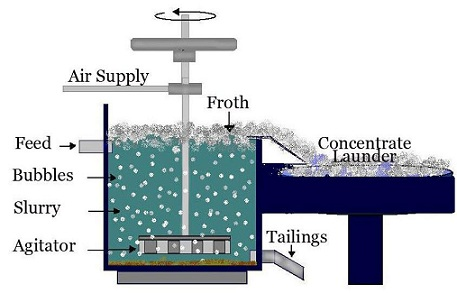
\includegraphics[width=0.8\textwidth]{images/mining_flow.jpg}
\caption{نمای کلی از فرآیند فرآوری مواد معدنی (خردایش، آسیاب، جدایش و آبگیری).}
\end{figure}

\section{آزمایشگاه تخصصی فرآوری مواد معدنی}

\subsection*{چالش‌های موجود}
در آزمایشگاه معمولاً باید نمونه را به دستگاه ببری و کلی زمان بگیرد. این فرآیند زمان‌بر و پرهزینه است.

\subsection*{نوآوری‌های هوش مصنوعی}

\subsubsection*{تشخیص ترکیب سنگ با عکس‌برداری}
با بینایی ماشین (AI) می‌توان از یک عکس میکروسکوپی یا حتی موبایل، رنگ، شکل و بافت سنگ را تحلیل کرد و حدس زد چه مقدار فلز داخل آن است. این روش سریع‌تر و کم‌هزینه‌تر از روش‌های سنتی است.

\subsubsection*{پیش‌بینی بهترین روش جداسازی}
در آزمایشگاه روش‌های مختلفی برای جدا کردن فلز وجود دارد (مثلاً شستشو با آب، مواد شیمیایی یا حرارت). AI می‌تواند با دیدن نتایج آزمایش‌های قبلی پیش‌بینی کند که کدام روش بیشترین بازده را می‌دهد.

\subsubsection*{تحلیل داده‌های آزمایشگاهی}
هوش مصنوعی می‌تواند داده‌های آزمایشگاهی (مثل درصد فلزات، شرایط دما و فشار، مصرف مواد شیمیایی) را تحلیل کند و الگوهای بهینه پیدا کند. مثلاً بعد از چند بار آزمایش، AI می‌فهمد که اگر سرعت همزن در فلوتاسیون ۲۰٪ کمتر باشد، بازیابی فلز بیشتر می‌شود.

\section{کارخانه پایلوت و صنعتی}

\subsection*{چالش‌های موجود}
\begin{itemize}
  \item ناپایداری کیفیت خوراک ورودی
  \item توقفات ناگهانی تجهیزات
  \item مصرف بالای انرژی و آب
\end{itemize}

\subsection*{نوآوری‌های هوش مصنوعی}

\subsubsection*{کنترل خودکار دستگاه‌ها}
کارخانه پر از دستگاه‌های آسیاب، جداکننده، پمپ و نوار نقاله است. سنسورها مدام دما، لرزش، سرعت و فشار را می‌خوانند. AI می‌تواند این داده‌ها را تحلیل کند و مثلاً بگوید سرعت آسیاب را کمی کم کن چون کیفیت خروجی افت کرده.

\subsubsection*{پیش‌بینی خرابی تجهیزات (نگهداری پیش‌بینانه)}
AI می‌تواند از روی صدای موتور یا لرزش یک دستگاه بفهمد که احتمالاً ۲ هفته دیگر خراب می‌شود و قبل از توقف کامل خط تولید، تعمیرش کنی.

\subsubsection*{بهینه‌سازی مصرف انرژی}
بعضی وقت‌ها تغییر کوچک در دما یا فشار می‌تواند مصرف برق را خیلی کم کند. AI می‌تواند بهترین تنظیمات را پیدا کند تا هم کیفیت خوب باشد هم هزینه کم.

\subsubsection*{کنترل کیفیت محصول}
وقتی فلز یا ماده فرآوری شده آماده می‌شود، AI می‌تواند با عکس‌برداری و اندازه‌گیری سریع بگوید آیا کیفیتش در محدوده استاندارد است یا نه.

\subsubsection*{تحلیل داده‌های پایلوت}
می‌شود داده‌های پایلوت را به AI داد تا الگوها را شناسایی کند و قبل از سرمایه‌گذاری بزرگ روی یک کارخانه صنعتی، بهترین روش را پیشنهاد بده. مثلاً AI پیش‌بینی کند «اگر فلوتاسیون با فلان ماده شیمیایی ادامه پیدا کند، در مقیاس صنعتی هزینه مواد مصرفی ۳۰٪ بیشتر می‌شود» → یعنی قبل از اینکه خرج میلیاردی شود، خطر دیده می‌شود.

\section{تجهیزات خط فرآوری}

هوش مصنوعی می‌تواند روی هر مرحله نظارت کند و بهترین شرایط را پیشنهاد بده. تجهیزات اصلی شامل:
\begin{itemize}
  \item سنگ‌شکن فکی و مخروطی \lr{→} برای خردایش اولیه سنگ
  \item آسیای گلوله‌ای و رادمیل \lr{→} برای خردایش نرم‌تر و رسیدن به پودر
  \item سلول فلوتاسیون ستونی و مکانیکی \lr{→} جداسازی کانی‌ها (مثلاً مس از باطله) با استفاده از حباب هوا
  \item مارپیچ همفری و میز لرزان \lr{→} برای جدایش ثقلی (بر اساس وزن مخصوص مواد)
  \item تیکنر و فیلتر پرس \lr{→} برای آب‌گیری و مدیریت باطله‌ها
\end{itemize}

\subsection{سنگ‌شکن (\lr{Crusher})}

\subsubsection*{چالش‌های اصلی}
\begin{itemize}
  \item فرسایش سریع فک‌ها و چکش‌ها \lr{→} هزینه بالا و توقف تولید
  \item تغییر ناگهانی سختی سنگ‌ها \lr{→} مصرف انرژی بیشتر یا شکستن تجهیزات
\end{itemize}

\subsubsection*{ایده‌های نوآورانه با AI}
\begin{itemize}
  \item \textbf{مدل پیش‌بینی هوشمند سختی سنگ:} استفاده از پردازش تصویر روی خوراک ورودی (قبل از ورود به سنگ‌شکن). قبل از خردایش، \lr{AI} عکس سنگ را می‌بیند و سختی را تخمین می‌زند \lr{→} تنظیم فشار و سرعت به صورت خودکار.
  \item \textbf{شنیدن صدای سنگ‌شکن (\lr{AI} صوتی):} از روی فرکانس صدا تشخیص می‌دهد کی سنگ غیرمعمول یا فلز وارد دستگاه شده \lr{→} هشدار فوری قبل از آسیب.
  \item \textbf{بهینه‌سازی شکل خوراک‌دهی:} با هوش مصنوعی جهت خوراک‌دهی اصلاح می‌شود تا توزیع یکنواخت سنگ باعث کاهش لرزش و افزایش عمر فک‌ها شود.
\end{itemize}

\begin{figure}[h!]
\centering
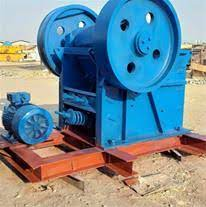
\includegraphics[width=0.6\textwidth]{images/crusher.jpg}
\caption{سنگ‌شکن فکی مورد استفاده در خردایش اولیه.}
\end{figure}

\subsection{آسیاب (\lr{Mill})}

\subsubsection*{چالش‌های اصلی}
\begin{itemize}
  \item مصرف وحشتناک انرژی
  \item گیرکردن یا بیش‌خردایش (\lr{Over-grinding}) \lr{→} اتلاف وقت و انرژی
\end{itemize}

\subsubsection*{ایده‌های نوآورانه با AI}
\begin{itemize}
  \item \textbf{بینایی ماشین برای تشخیص اندازه ذرات لحظه‌ای:} دوربین \lr{AI} روی خروجی آسیاب \lr{→} بلافاصله اندازه ذرات را تخمین می‌زند و سرعت آسیاب یا اندازه گلوله‌ها را تنظیم می‌کند.
  \item \textbf{بهینه‌سازی دینامیکی گلوله‌ها:} الگوریتم \lr{AI} محاسبه می‌کند چه ترکیبی از گلوله‌های کوچک/بزرگ بهترین بازدهی را دارد \lr{→} سفارش هوشمند گلوله برای خط تولید.
  \item \textbf{مدل‌سازی مصرف انرژی + کیفیت محصول:} با یادگیری تقویتی (\lr{Reinforcement Learning}) \lr{→} آسیاب یاد می‌گیرد چطور با کمترین انرژی، بهترین خروجی را بدهد.
\end{itemize}

\begin{figure}[h!]
\centering
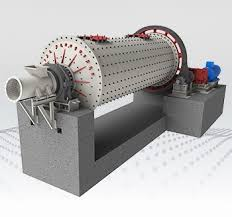
\includegraphics[width=0.6\textwidth]{images/mill.jpeg}
\caption{آسیاب گلوله‌ای در مدار فرآوری مواد معدنی.}
\end{figure}

\subsection{سلول فلوتاسیون (\lr{Flotation Cell})}

\subsubsection*{چالش‌های اصلی}
\begin{itemize}
  \item تغییر کیفیت سنگ → تنظیم دستی کف‌سازها و کلکتورها
  \item خطای انسانی زیاد در تشخیص "کیفیت کف"
\end{itemize}

\subsubsection*{ایده‌های نوآورانه با AI}
\begin{itemize}
  \item \textbf{بینایی ماشین برای آنالیز کف فلوتاسیون:} \lr{AI} از روی رنگ، شکل و پایداری کف، کیفیت فرآیند را تحلیل می‌کند \lr{→} بدون نیاز به اپراتور.
  \item \textbf{مدل‌های چندعاملی (\lr{Multi-agent AI}):} برای کنترل تزریق هوا، مواد شیمیایی و همزن به صورت همزمان \lr{→} یکپارچه‌سازی کل فرآیند.
  \item \textbf{مدل یادگیری از تجربه (\lr{Transfer Learning}):} اگر معدن \lr{A} روی سنگ مس کار کرده، تجربه مدل \lr{AI} برای معدن \lr{B} هم قابل استفاده باشد \lr{→} تسریع در تنظیمات.
\end{itemize}

\begin{figure}[h!]
\centering
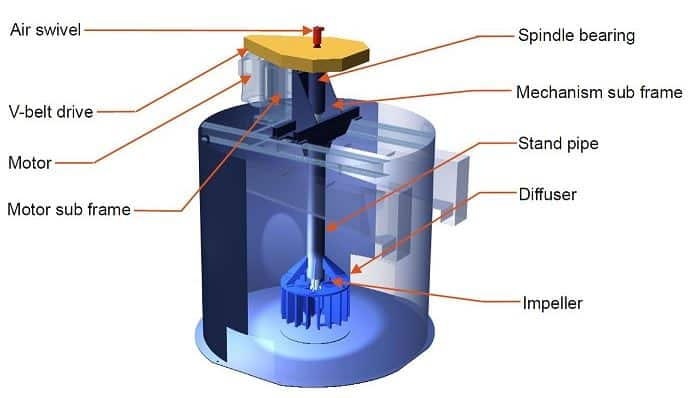
\includegraphics[width=0.6\textwidth]{images/flotation_cell.jpg}
\caption{سلول‌های فلوتاسیون مکانیکی برای جداسازی کانی‌ها.}
\end{figure}

\subsection{تجهیزات جدایش ثقلی (مارپیچ، میز لرزان)}

\subsubsection*{چالش‌های اصلی}
\begin{itemize}
  \item تغییر ناگهانی اندازه یا چگالی خوراک → افت کیفیت محصول
  \item وابستگی شدید به تجربه اپراتور
\end{itemize}

\subsubsection*{ایده‌های نوآورانه با AI}
\begin{itemize}
  \item \textbf{تشخیص لحظه‌ای مسیر حرکت ذرات:} با دوربین حرارتی یا \lr{RGB} \lr{→} \lr{AI} اصلاح زاویه مارپیچ یا میز را به‌صورت خودکار پیشنهاد می‌دهد.
  \item \textbf{ترکیب \lr{AI} با \lr{CFD} (شبیه‌سازی سیالات):} برای پیش‌بینی رفتار ذرات در شرایط مختلف خوراک \lr{→} تنظیم بهینه تجهیزات.
  \item \textbf{سیستم تطبیقی \lr{Real-time}:} میز لرزان یا مارپیچ به طور خودکار خودش را متناسب با خوراک ورودی تنظیم می‌کند.
\end{itemize}

\begin{figure}[h!]
\centering
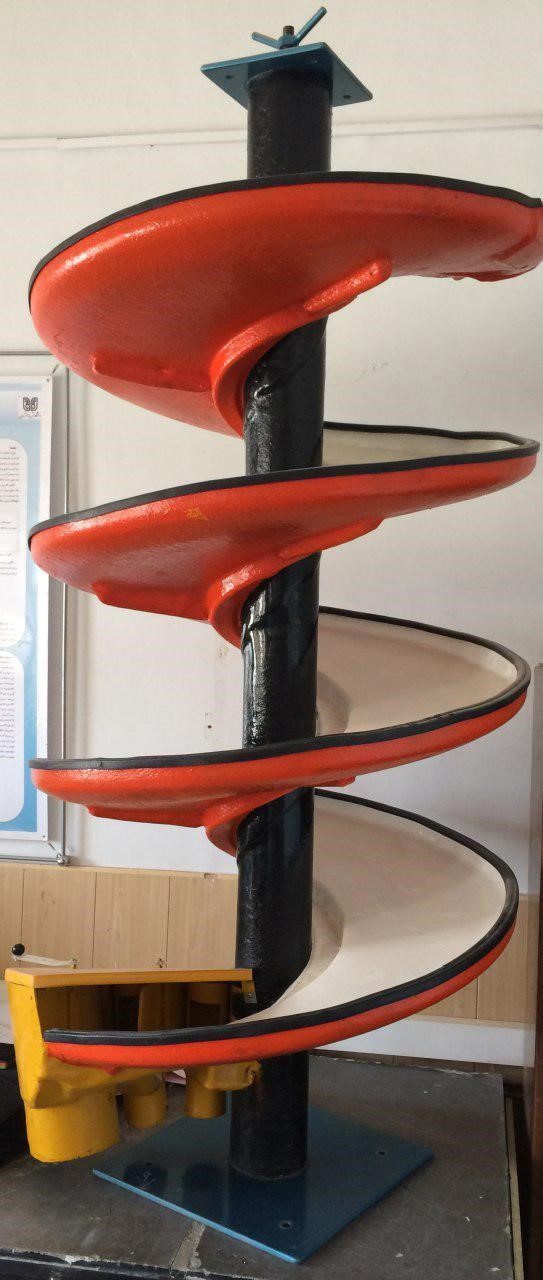
\includegraphics[width=0.6\textwidth]{images/gravity_separation.jpg}
\caption{میز لرزان برای جدایش ثقلی مواد معدنی.}
\end{figure}

\subsection{تیکنر و فیلتر پرس (\lr{Thickener \& Filter Press})}

\subsubsection*{چالش‌های اصلی}
\begin{itemize}
  \item بازیافت کم آب
  \item گرفتگی فیلترها و نیاز به شستشوی مکرر
  \item کیفیت پایین لجن
\end{itemize}

\subsubsection*{ایده‌های نوآورانه با AI}
\begin{itemize}
  \item \textbf{مدل \lr{AI} برای پیش‌بینی گرفتگی فیلتر:} از روی فشار، دما و جریان \lr{→} قبل از توقف خط.
  \item \textbf{بهینه‌سازی مصرف فلوکولانت:} \lr{AI} از روی کیفیت خوراک مقدار دقیق ماده شیمیایی را تعیین می‌کند.
  \item \textbf{مدل‌سازی ریسک سد باطله:} \lr{AI} از داده‌های خروجی تیکنر (غلظت لجن و دبی آب) استفاده می‌کند تا خطر تجمع بیش از حد یا ناپایداری سد را هشدار بدهد.
\end{itemize}

\begin{figure}[h!]
\centering
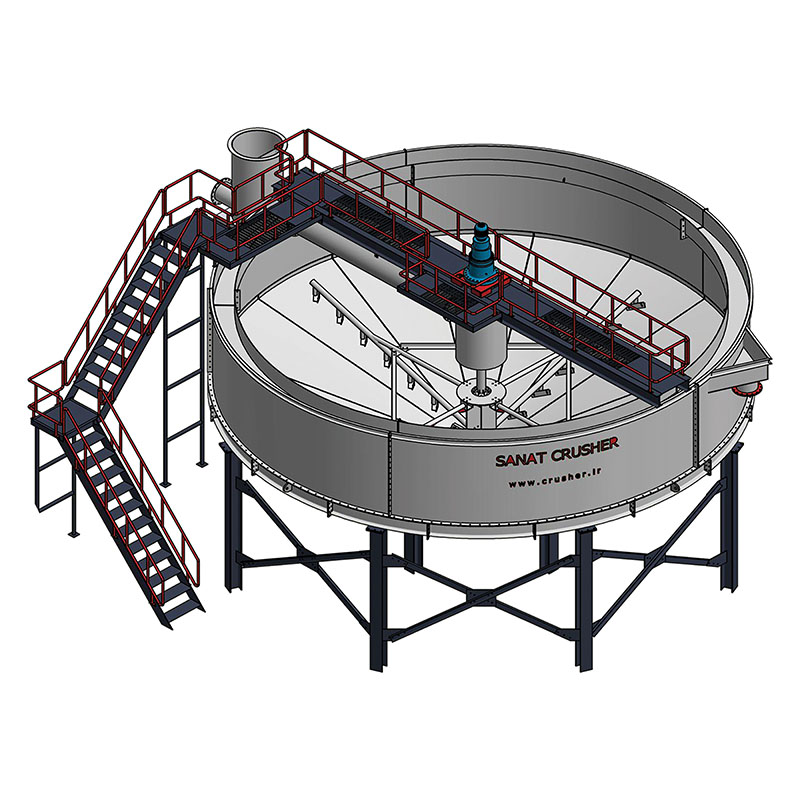
\includegraphics[width=0.6\textwidth]{images/thickener.jpg}
\caption{تیکنر صنعتی برای آبگیری و بازیافت آب.}
\end{figure}

\section*{جمع‌بندی}
کاربرد هوش مصنوعی در فرآوری مواد معدنی نه‌تنها باعث افزایش بازده و کاهش هزینه‌ها می‌شود، بلکه می‌تواند در ارتقای ایمنی و پایداری محیط‌زیستی نیز نقش کلیدی ایفا کند. 
این نوآوری‌ها مسیری نو برای حرکت معادن کشور به سمت معدن‌کاری هوشمند (\lr{Smart Mining}) فراهم می‌کنند.
%تحقیقات و نوآوری‌های هوش مصنوعی در فرآوری مواد معدنی
% !TeX root=main.tex
\chapter{پروژه‌های مهم منتخب}

\section*{اپلیکیشن فاکتور}
«فاکتور» یک اپلیکیشن حسابداری و مدیریت مالی است که توسط اینجانب طراحی و توسعه داده شده و تاکنون بیش از ۱۲۰{,}000 نصب فعال در کافه‌بازار داشته است. 
این اپلیکیشن بر پایه فریم‌ورک \lr{Flutter} توسعه یافته و از معماری‌های مدرن (Clean Architecture, Riverpod) بهره می‌برد. 
چالش اصلی این پروژه مدیریت بهینه داده‌ها، پشتیبانی از حالت آفلاین، و مقیاس‌پذیری برای تعداد بالای کاربران بود که با طراحی دقیق و استفاده از فناوری‌هایی مانند \lr{ObjectBox} و \lr{Retrofit} حل شد. 

\section*{پایان‌نامه کارشناسی‌ارشد}
پایان‌نامه من بر محور ترکیب اپلیکیشن‌های اندرویدی با الگوریتم‌های هوش مصنوعی و شبکه‌های عصبی متمرکز بوده است. 
در این پروژه از معماری‌های مختلف یادگیری عمیق (\lr{CNN}، \lr{RNN}، \lr{Transfer Learning}) استفاده شد تا قابلیت هوشمندسازی اپلیکیشن‌ها در حوزه‌های مختلف مانند دسته‌بندی تصاویر و تحلیل داده‌های متنی بررسی شود. 
این تجربه موجب افزایش تسلط من بر چارچوب‌های یادگیری عمیق و کاربرد آن‌ها در اپلیکیشن‌های واقعی شد. 

\section*{پروژه‌های پردازش تصویر دانشگاهی}
در طول دوران تحصیل، روی چندین پروژه پردازش تصویر کار کرده‌ام. 
این پروژه‌ها شامل شناسایی الگوها در تصاویر میکروسکوپی، تشخیص اشیاء و آنالیز داده‌های تصویری در محیط‌های آزمایشگاهی بوده‌اند. 
برای این کار از کتابخانه‌هایی مانند \lr{OpenCV} و شبکه‌های عصبی کانولوشنی استفاده کردم. 
این پروژه‌ها زیربنای علاقه‌مندی من به کاربردهای نوآورانه هوش مصنوعی در حوزه معدن شدند. 

\section*{پکیج اختصاصی PrimaryKit}
برای بهبود سرعت توسعه در پروژه‌های مختلف، یک پکیج اختصاصی به نام \lr{PrimaryKit} طراحی و توسعه داده‌ام. 
این پکیج شامل کامپوننت‌های مشترک (مانند دکمه‌ها و فیلدهای متنی) بوده و در پروژه‌های متعدد \lr{Flutter} استفاده شده است. 
این اقدام علاوه بر صرفه‌جویی در زمان توسعه، موجب افزایش هماهنگی در کدها و استانداردسازی پروژه‌ها شد.
%پروژه‌های مهم منتخب
% !TeX root=main.tex
\chapter{جمع‌بندی و پیشنهادات آینده}

\section*{جمع‌بندی}
در این سند نشان داده شد که استفاده از هوش مصنوعی می‌تواند در تمامی مراحل فرآوری مواد معدنی، از آزمایشگاه گرفته تا کارخانه صنعتی، نقش کلیدی ایفا کند. 
نوآوری‌های مبتنی بر هوش مصنوعی، مانند پردازش تصویر برای تشخیص ترکیب سنگ‌ها، نگهداری پیش‌بینانه تجهیزات، بهینه‌سازی مصرف انرژی و آب، و کنترل هوشمند کیفیت محصول، همگی می‌توانند موجب افزایش بهره‌وری و کاهش هزینه‌ها شوند. 
علاوه بر این، کاربرد \lr{AI} به ارتقای ایمنی، کاهش توقفات ناگهانی، و حرکت به سمت معدن‌کاری هوشمند کمک می‌کند.

\section*{پیشنهادات آینده}
\begin{itemize}
  \item \textbf{ایجاد پایگاه داده ملی فرآوری معدنی:} 
  داده‌های واقعی از معادن مختلف ایران جمع‌آوری و به صورت استاندارد ذخیره شوند تا الگوریتم‌های \lr{AI} بتوانند بر اساس داده‌های متنوع‌تر آموزش ببینند.
  
  \item \textbf{ترکیب \lr{IoT} و \lr{AI}:} 
  استفاده از حسگرهای اینترنت اشیا (\lr{IoT}) در کنار الگوریتم‌های یادگیری ماشین برای پایش لحظه‌ای تجهیزات و خطوط تولید.
  
  \item \textbf{شبیه‌سازی دیجیتال (\lr{Digital Twin}):} 
  ایجاد مدل‌های دیجیتال از تجهیزات کلیدی مانند آسیاب یا سلول فلوتاسیون که امکان تست مجازی تنظیمات مختلف را پیش از اعمال در دنیای واقعی فراهم می‌کند.
  
  \item \textbf{بهینه‌سازی زیست‌محیطی:} 
  استفاده از \lr{AI} برای پایش و پیش‌بینی پایداری سدهای باطله، کاهش مصرف مواد شیمیایی و مدیریت پساب‌ها.
  
  \item \textbf{همکاری میان‌رشته‌ای:} 
  ترکیب تخصص‌های معدن، مهندسی شیمی و هوش مصنوعی برای خلق راه‌حل‌های نوآورانه در صنایع معدنی.
\end{itemize}

\section*{نتیجه}
حرکت به سمت معدن‌کاری هوشمند تنها یک انتخاب فناورانه نیست، بلکه ضرورتی برای پایداری اقتصادی و زیست‌محیطی صنعت معدن در ایران محسوب می‌شود. 
با سرمایه‌گذاری در این حوزه، می‌توان آینده‌ای را متصور شد که در آن معادن کشور با کمترین هزینه و بیشترین بازدهی به بهره‌برداری برسند.
%جمع‌بندی و پیشنهادات آینده
\end{document}
%% End of file `main.tex'.
